% -----------------------------*- LaTeX -*------------------------------
\documentclass[11pt]{report}
\usepackage{scribe_ds603}
\usepackage{graphicx} 

\begin{document}

\scribe{Anurag Deshpande}		% required
\lecturenumber{9}			% required, must be a number
\lecturedate{12th September}		% required, omit year

\maketitle

% ----------------------------------------------------------------------

\section{Attack Strategy: Bilevel Optimization}

Bilevel optimization ~\cite{zhang2023introduction}is a powerful and general framework for formulating data poisoning attacks. It is applicable across various scenarios, including indiscriminate, targeted, clean-label, and backdoor attacks. The primary requirement for this strategy is that the attacker has access to the training data and the model architecture.

\subsection{General Formulation}
The attack is structured as a nested optimization problem. The outer loop optimizes the poisoned data to achieve the attacker's goal, while the inner loop simulates the training of the model on this data. We define the following notation:
\begin{itemize}
    \item $D_{train}$: The full original training dataset.
    \item $D_p$: The subset of training data that can be poisoned by the attacker.
    \item $D_c$: The clean, unmodifiable portion of the training data.
    \item $D_v$: A clean validation set, drawn i.i.d. from the true data distribution, used to define the attacker's objective.
    \item $M(\cdot)$: A manipulation function that defines the set of allowed perturbations.
    \item $\theta \in \mathbb{R}^d$: The model parameters. We denote parameters trained on poisoned data as $\tilde{\theta}_p$.
\end{itemize}
The general bilevel optimization problem for a targeted attack is formulated as:
\begin{align}
    \underset{\tilde{D}_p \in M(D_p)}{\text{maximize}} &\quad \hat{L}(D_v, \tilde{\theta}_p) \label{eq:outer_problem} \\
    \sbjto &\quad \tilde{\theta}_p \in \underset{\theta}{\text{argmin}} \quad \hat{L}(D_c \cup \tilde{D}_p, \theta) \label{eq:inner_problem}
\end{align}
Here, we maximize the loss on the validation set $D_v$ to cause misclassification of target examples.

\subsection{Indiscriminate Poisoning}
The goal is to find a poisoned dataset $\tilde{D}_{\rho}$ that maximizes the loss on a clean dataset when the model is trained on the poisoned data.
\begin{gather}
    \maximize_{\tilde{D}_{\rho} \in M(D_{\rho})} \mathbb{E}_{\tilde{z} \sim P^*}[l(\tilde{z}, \tilde{h})] \\
    \sbjto \quad \tilde{h} \in \argmin_{h} L(D_c \cup \tilde{D}_{\rho}, h) \nn
\end{gather}

\subsection{Targeted Poisoning}
In targeted poisoning, the attacker aims to cause misclassification for a specific target instance.
\begin{gather}
    \minimize_{\tilde{D}_{\rho} \in M(D_{\rho})} \hat{L}(D_v, \tilde{h}) \\
    \sbjto \quad \tilde{h} \in \argmin_{h} \hat{L}(D_c \cup \tilde{D}_{\rho}, h) \nn
\end{gather}

\subsection{Backdoor Attacks}
Backdoor attacks involve inserting a trigger into the training data. The model learns to associate the trigger with a specific target label.
\begin{gather}
    \minimize_{\tilde{D}_{\rho} \in M(D_{\rho})} \hat{L}(D_c \cup \tilde{D}_{\rho}, h) \\
    \sbjto \quad \tilde{h} \in \argmin_{h} \hat{L}(D_c \cup \tilde{D}_{\rho}, h) \nn
\end{gather}
It is important to note that the triggers used during training and testing are usually the same.

\subsection{Solving the Bilevel Optimization Problem}
A key question is how to solve the bilevel optimization problem efficiently ~\cite{ye2022bomebileveloptimizationeasy}. Let's simplify the notation. Consider a single poison point $(\vec{x}^p, y^p)$. We want to solve:\\
\begin{gather}
    \argmax_{\tilde{D}_p \in M(D_p)} 1/n_v \sum_{i=1}^{n_v} l(z_i, \vec\theta_p) \\
    \sbjto \quad \theta_p \in \argmin_{\theta} \frac{1}{n_c+n_p} \left( \sum_{i=1}^{n_c} l(z_i, \vec\theta_p) + \sum_{i=1}^{n_p} l({z}^*_i, {y}^*_i), \vec\theta_p) \right) \nn
\end{gather}

%simplification
\begin{itemize}
    \item \textbf{Single Poison Point}: We assume the adversary controls only a single poison point $(\bm{x}_p, y_p)$ and fixes the poison label $y_p$ throughout the attack. The optimization is performed over the features $\bm{x}_p$.
    \item \textbf{Loss Function Properties}: The loss function $l(z, \theta)$ is assumed to be twice differentiable and convex with respect to the parameters $\theta$, ensuring the Hessian is positive definite ($\nabla^2_{\theta} l(z, \theta) \succ 0$).
\end{itemize}

%gradient ascent - cut from text


\subsection{Gradient Ascent Attack}
With these assumptions, the outer maximization problem for the single poison point can be reformulated, and simply stated, and becomes:
\begin{equation}
    \underset{\bm{x}_p \in M(\cdot)}{\text{maximize}} \quad \hat{L}(D_v, \tilde{\theta}_p(\bm{x}_p))
\end{equation}

We can solve this using \textbf{Projected Gradient Ascent}. At each step $t$, the poison features $\bm{x}_p$ are updated as follows:

\begin{equation}
    \vec{x}_t^p = \vec{x}_{t-1}^p + \eta \nabla_{\vec{x}_{t-1}^p} \hat{L}(D_v, \tilde{\theta}_p(\vec{x}_{t-1}^p))
\end{equation}
where $\eta$ is the learning rate, and the updated point is projected back into the allowed manipulation set (e.g., to maintain image validity). The main challenge is computing the gradient $\nabla_{\bm{x}_p} \hat{L}(\cdot)$.


%nice equation below

\subsection{Chain Rule and Implicit Differentiation}
Using the chain rule, the gradient of the validation loss w.r.t. the poison data $\bm{x}_p$ is:
\begin{equation}
    \nabla_{\bm{x}_p} \hat{L}(D_{v}, \tilde{\theta}_p(\bm{x}_p)) = \underbrace{\left( \frac{\partial \tilde{\theta}_p(\bm{x}_p)}{\partial \bm{x}_p} \right)^T}_{\text{Term 1: Jacobian}} \underbrace{\nabla_{\tilde{\theta}_p} \hat{L}(D_v, \tilde{\theta}_p(\bm{x}_p))}_{\text{Term 2: Validation Gradient}}
    \label{eq:chain_rule}
\end{equation}
Term 2 is easy to compute via backpropagation. Term 1, the Jacobian, describes how the learned parameters change with respect to the poison data. To compute it, we use the \textbf{stationarity condition} from the inner optimization problem (Eq. \ref{eq:inner_problem}), which states that the gradient of the training loss at the optimal parameters $\tilde{\theta}_p$ is zero:
\begin{equation}
    \nabla_{\tilde{\theta}_p} \hat{L}(D_c \cup \{(\bm{x}_p, y_p)\}, \tilde{\theta}_p(\bm{x}_p)) = 0
\end{equation}
By the implicit function theorem, we can differentiate this entire equation with respect to $\bm{x}_p$:
\begin{equation}
    \frac{d}{d\bm{x}_p} \left[ \nabla_{\tilde{\theta}_p} \hat{L}(D_c \cup \{z_p\}, \tilde{\theta}_p) \right] = 0
\end{equation}
Applying the total derivative yields:
\begin{equation}
    \nabla_{\bm{x}_p} \nabla_{\tilde{\theta}_p} \hat{L}(D_{train}, \tilde{\theta}_p) + \left(\frac{\partial \tilde{\theta}_p}{\partial \bm{x}_p}\right)^T \nabla_{\tilde{\theta}_p}^2 \hat{L}(D_{train}, \tilde{\theta}_p) = 0
\end{equation}
Let $H_{\tilde{\theta}} = \nabla_{\tilde{\theta}_p}^2 \hat{L}(D_{train}, \tilde{\theta}_p)$ be the Hessian of the training loss. We can now solve for the Jacobian term:
\begin{equation}
    \left(\frac{\partial \tilde{\theta}_p}{\partial \bm{x}_p}\right)^T = - \left[ \nabla_{\bm{x}_p} \nabla_{\tilde{\theta}_p} \hat{L}(D_{train}, \tilde{\theta}_p) \right] H_{\tilde{\theta}}^{-1}
    \label{eq:jacobian_final}
\end{equation}
Since $\bm{x}_p$ only appears in one term of the loss, this simplifies to $\nabla_{\bm{x}_p} \nabla_{\tilde{\theta}_p} l(z_p, \tilde{\theta}_p)$. Substituting Eq. \ref{eq:jacobian_final} into the chain rule (Eq. \ref{eq:chain_rule}) gives the final expression for the attack gradient. Further steps are possible to speed up computation ~\cite{koh2017understanding}

%% handwritten finish

\begin{figure}[!h]
    \centering
    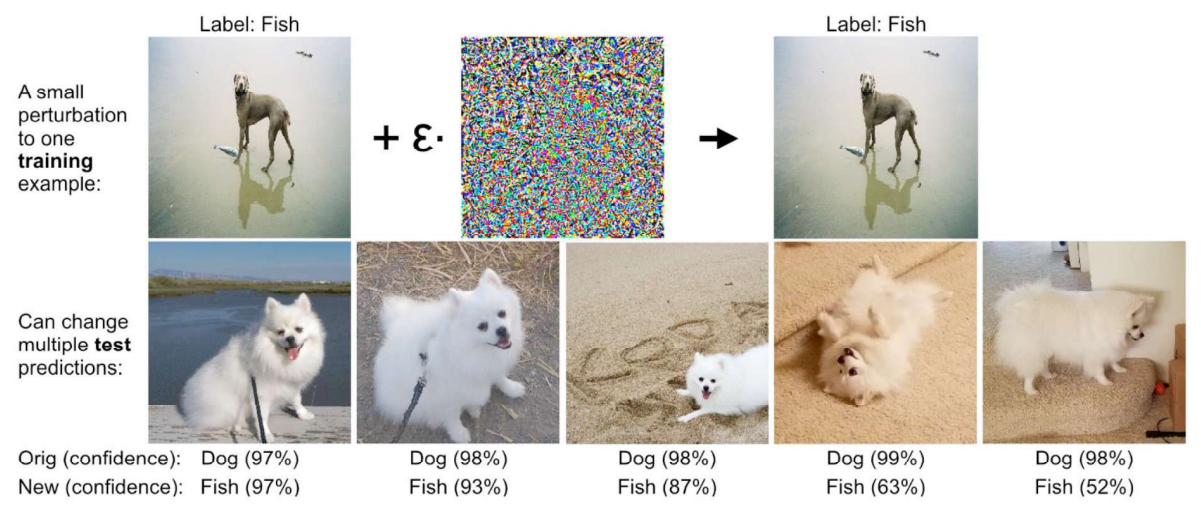
\includegraphics[width=0.8\textwidth]{results_bilevel.png}
    \caption{A small perturbation to one training example can change multiple test predictions. The model used is an Inception architecture where only the last layer is retrained at each iteration.}
    \label{fig:bilevel_results}
\end{figure}

\section{Attack Strategy: Feature Collision}

This is a targeted attack applicable in clean and backdoor scenarios, requiring both data and model access, where the model can only be fine-tuned. The attacker aims to create a poison instance that has a similar feature representation to a target instance.

The poison point $\vec{x}^p$ is found by solving the following optimization problem:
\begin{align}
    \vec{x}^p = \argmin_{\vec{x} \in \mathbb{R}^k} [||\phi(\vec{x}) - \phi(\vec{x}^t)||_2^2 + \lambda ||\vec{x} - \vec{x}^c||_2^2] \nn
\end{align}
where $\phi$ is a known feature extractor, $\vec{x}^t$ is the target instance, and $\vec{x}^c$ is a clean base instance.

\begin{figure}[!h]
    \centering
    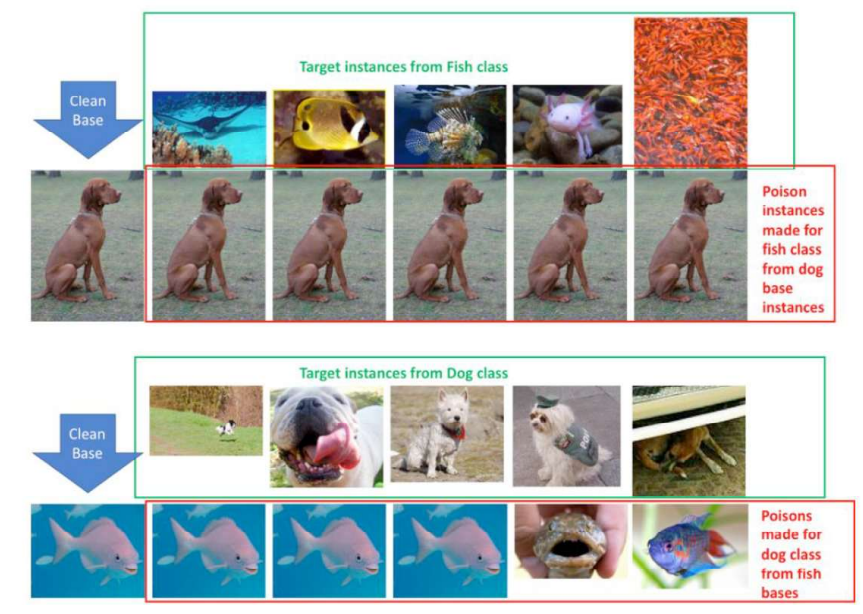
\includegraphics[width=0.9\textwidth]{results_collision.png}
    \caption{Results of feature collision attacks. (a) shows sample target and poison instances. (b) shows that poisoned models misclassify the target with high confidence.}
    \label{fig:collision_results}
\end{figure}


\section{Attack Strategy: Gradient Alignment}
This is a targeted attack for clean and backdoor scenarios that requires both data and model access. The core idea is to craft a poisoned image whose gradient aligns with the gradient of the loss for the target image. ~\cite{truong2025addressinggradientmisalignmentdataaugmented}
\\

Thus, the optimization problem is formulated as:

\begin{gather}
    \underset{\tilde{D_p} \in M(D_p)}{\min} \quad 1 - \frac{\langle \nabla_{\theta} l(h_{\theta}(\vec{x}^t), y^p), \nabla_{\theta} \hat{L}(\tilde{D}_p, \vec{\theta}) \rangle}{||\nabla_{\theta}l(h_{\theta}(\vec{x}^t), y^p)|| \cdot ||\nabla_{\theta}\hat{L}(\tilde{D}_p, \vec{\theta})||}
\end{gather}

where $h_{\theta}$ is a pre-trained clean model.

\begin{figure}[!h]
    \centering
    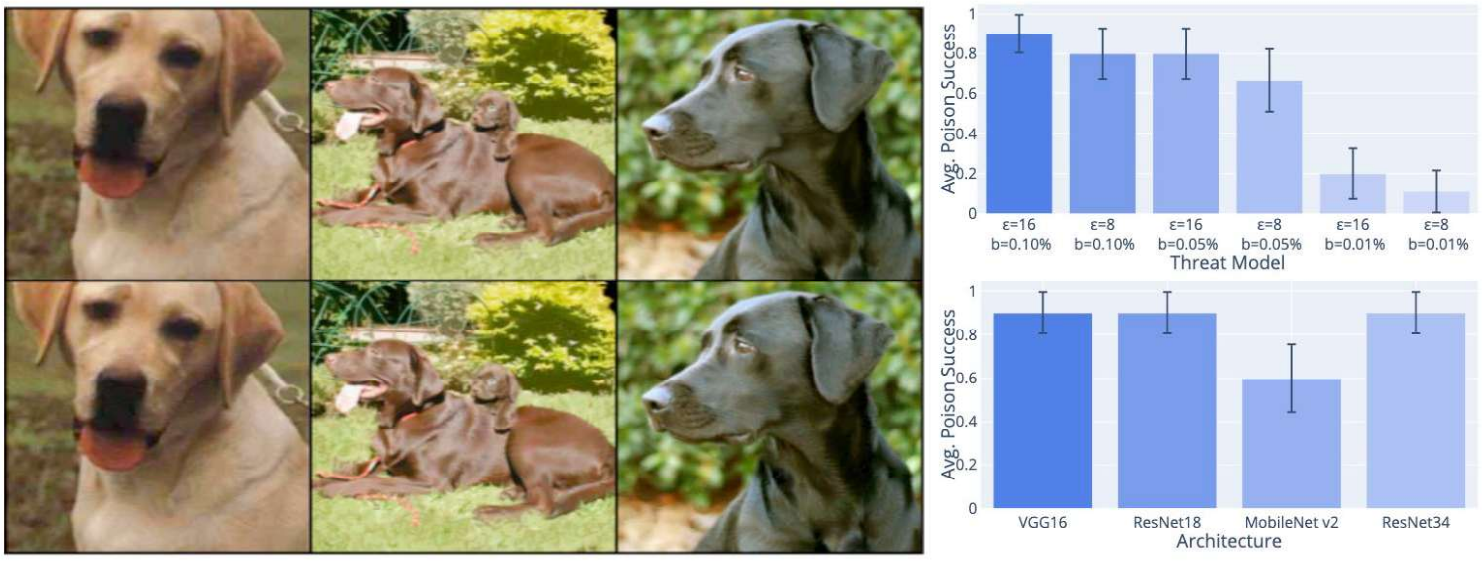
\includegraphics[width=0.8\textwidth]{results_gradient.png}
    \caption{Poisoning ImageNet using Gradient Alignment. The left panel shows clean images and their poisoned counterparts. The right panels show the success rate for different poison budgets and model architectures.}
    \label{fig:gradient_results}
\end{figure}


\section{Empirical considerations}
\begin{itemize}
    \item \textbf{Poison fraction sensitivity:} Typical curves show test accuracy vs poison fraction (0\% to 20\%), with steep drops in some regimes.
    \item \textbf{Label flip vs clean-label:} Label-flip often simpler but easier to detect; clean-label often requires optimization that preserves perceptual similarity.
    \item \textbf{Defense notes:} Common defenses include data sanitization, robust training, and influence-based detection.
\end{itemize}



\bibliographystyle{plain}
\bibliography{refs}

\end{document}
